\subsubsection{Data Collection}
In section~\ref{subsubsec:intro-data-collection} we define the tools used to collect data, this section will elaborate
on that to provide a full test suite for data collection.

\subsubsection{Experimental Space}
The experimentation in this paper are being performed on a laptop with the battery removed, the specifications are as
follows:

\textbf{Laptop}: Lenovo ThinkPad P1

\textbf{CPU}: Intel(R) Core(TM) i7-8850H CPU @ 2.60GHz

\textbf{Memory}: 32GB

\textbf{Disk}: 500GB SAMSUNG MZVLB512HAJQ-000L7

\textbf{OS}: Ubuntu 23.10

\textbf{Kernel}: 6.5.0-28-generic

\subsubsection{Polling Frequency}
The first step in data collection is to determine the frequency at which we will poll the system, this is important as
higher poll rates will affect the system more, while providing more accurate data.
Intel claims an update frequency of approximately 1 millisecond\cite{RAPLInterface}, providing an upper limit for viable
frequency, however the value that we choose will likely be lower than this, due to the time required to read from the
RAPL interface.
As it is impossible to guarantee exact intervals (to within microseconds), we will normalize all results to
Joules/second, this will also prevent higher poll frequencies from having lower energy readings, allowing for easeier
comparisons of the true invasiveness of the polling system.

In addition to finding the optimal polling frequency, this section will provide a baseline control dataset that can be
compared against future data.

\textbf{Rate - 1s}
A rate of 1 second produces unremarkable results, as there is a lack of comparison so far.

\begin{figure}[H]
    \centering
    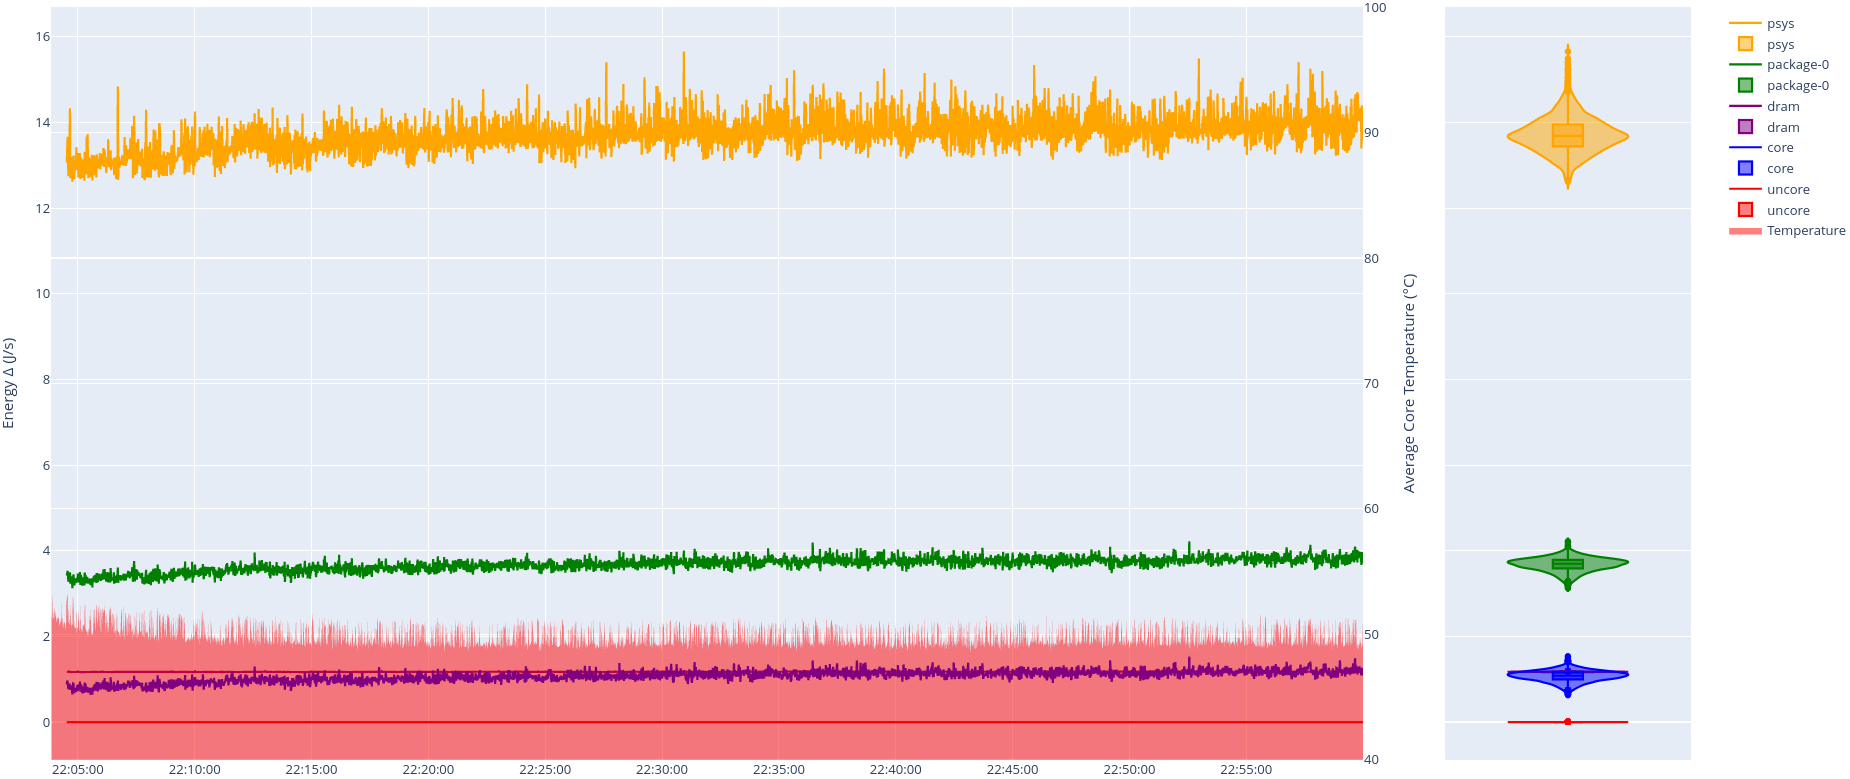
\includegraphics[width=15cm]{figures/implementation/control_sytemd10}
    \caption{Polling the powercap interface at a rate of every second for an hour; psys stats are: min - 12.61, max - 15.65, mean - 13.70, std - 0.41}
    \label{fig:systemd10ratetest}
\end{figure}

\textbf{Rate - 0.5s}
A rate of 0.5 seconds has a noticeable increase in power usage, however variance is slightly lower, this could either be
due to random chance, or it may indicate that there is a pattern to the volatility of RAPL's power readings, which
suggest the possibility of modeling the baseline pattern of the system to predict future power usage.
This rate also exposes a cyclical pattern to temperature, which may be useful for future analysis.

\begin{figure}[H]
    \centering
    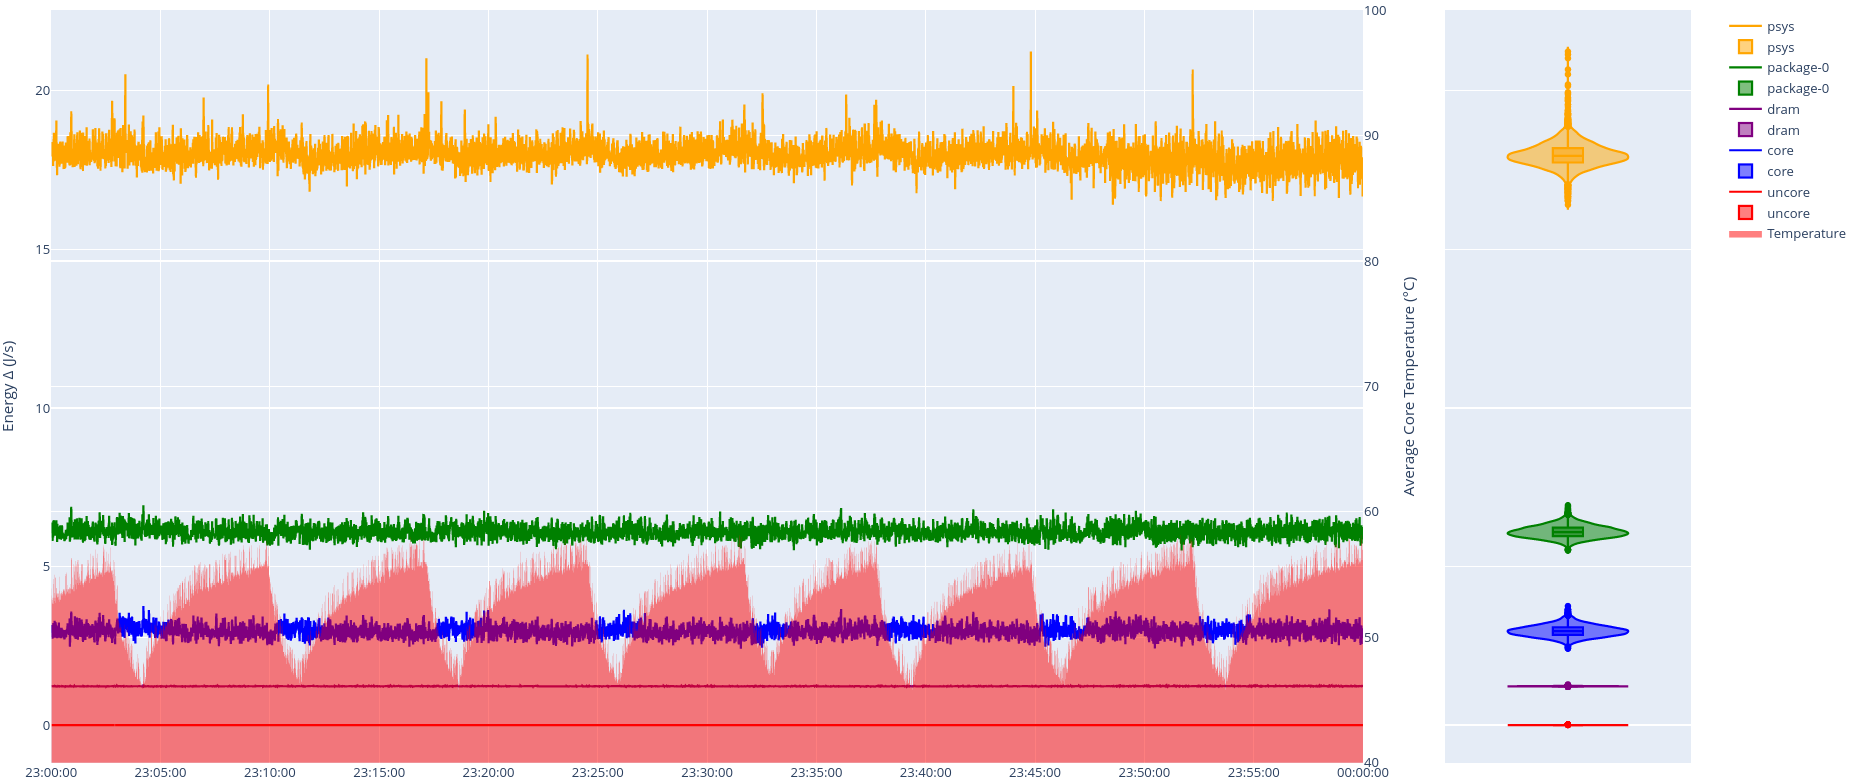
\includegraphics[width=15cm]{figures/implementation/control_systemd05}
    \caption{Polling the powercap interface at a rate of every 0.5 seconds for an hour; psys stats are: min - 16.41, max - 21.24, mean - 17.97, std - 0.38}
    \label{fig:systemd05ratetest}
\end{figure}

\textbf{Rate - 0.2s}
A rate of 0.2 seconds uses almost double the energy of the 1 second rate, and has much higher variance, making it the
worst choice for a polling rate.

\begin{figure}[H]
    \centering
    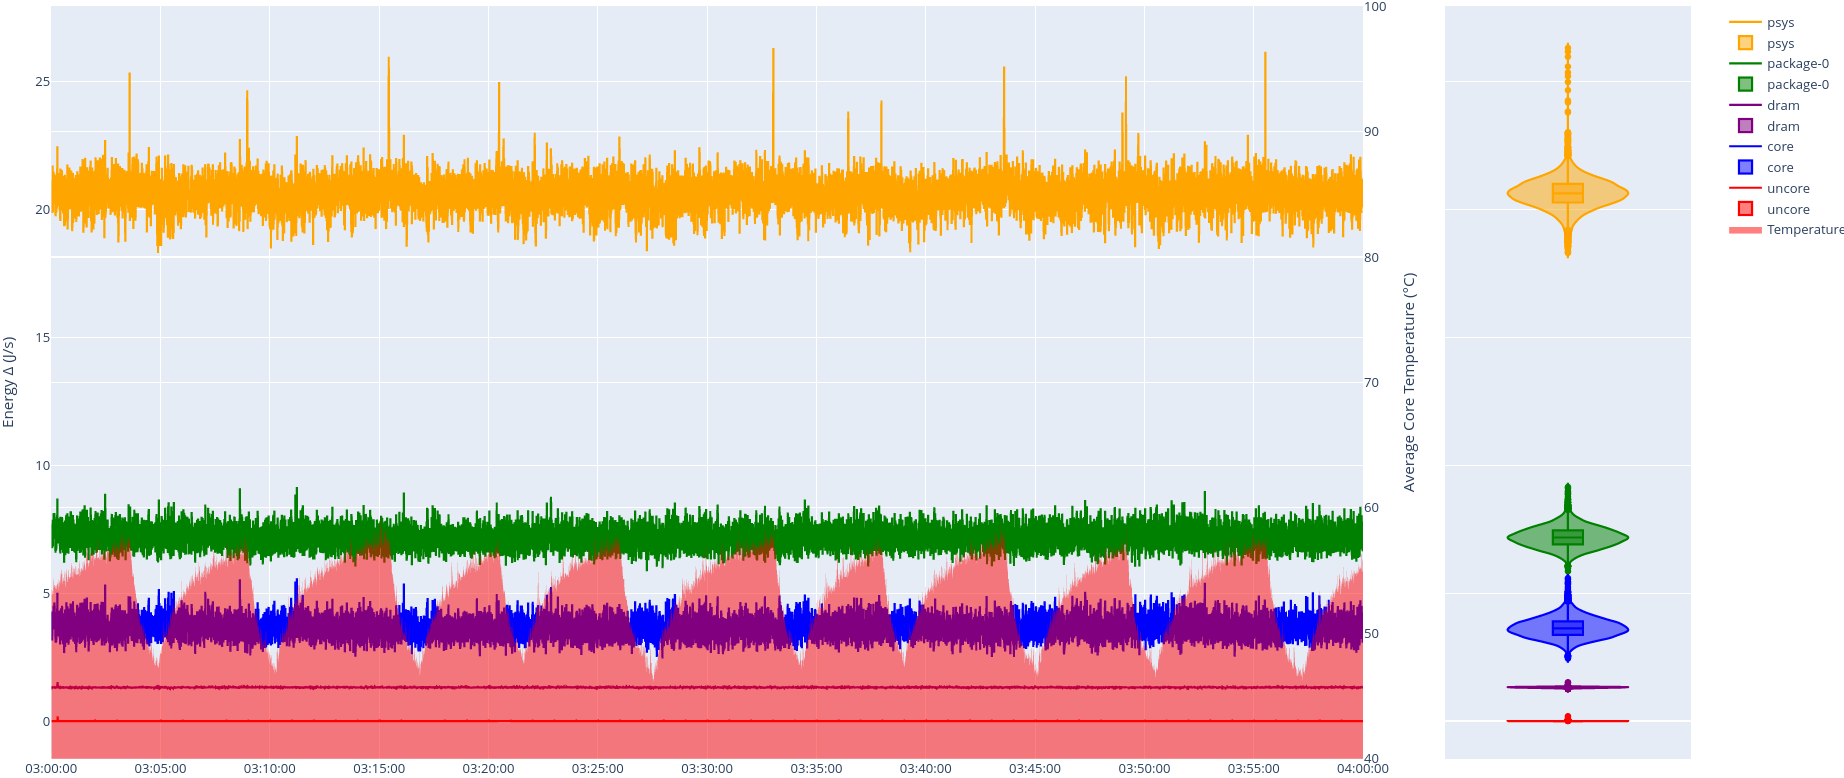
\includegraphics[width=15cm]{figures/implementation/control_systemd02}
    \caption{Polling the powercap interface at a rate of every 0.2 seconds for an hour; psys stats are: min - 18.29, max - 26.30, mean - 20.61, std - 0.58}
    \label{fig:systemd02ratetest}
\end{figure}


\textbf{Conclusion}

Unfortunately increasing the rate past 0.2 seconds appears to crash the systemd process, and has been deemed not viable
for experimentation.
As results are relative, we choose the polling rate of 0.5 seconds, as it provides a good balance between invasiveness
and repeatable patterns - and better models temperature change.
Readers repeating the process may also want to use these results to extrapolate the energy cost of the polling system -
this can be done by taking the difference between the mean of the 0.5s rate and the 1s rate, and then multiplying this
that difference by 2 (note that this is unlikely to be accurate, and is disproved by our results where the difference
between 1 and 0.5 should be smaller than the difference between 0.5 and 0.2).

Lastly, RAPL occasionally resets the powercap interface to zero readings - this interferes with results, as it is no
longer possible to simply compare the power reading before and after results.
Due to the nature of powercap updates, we will never receive a zero value, so the current process is to subtract the
first power usage value from the maximum, and then add the final value - it is important to note that this approach will
not work for experiments that run long enough to have two or more updates.

\subsubsection{Experiment Process}
As even the most sanitised systems are unlikely to have a completely stable power usage, we will need to have multiple
runs of each.
For this report we have chosen to run each experiment 10 times, then average results deemed to not be outliers -
outliers will be identified by unexplained rises in temperature, or large deviation from the mean.
There will be a 10-minute gap for each experiment, this length of time has been chosen simply as a convenient length of
time for plotting results, allowing for faster visual inspection of the data.